\documentclass[twoside]{book}

% Packages required by doxygen
\usepackage{fixltx2e}
\usepackage{calc}
\usepackage{doxygen}
\usepackage[export]{adjustbox} % also loads graphicx
\usepackage{graphicx}
\usepackage[utf8]{inputenc}
\usepackage{makeidx}
\usepackage{multicol}
\usepackage{multirow}
\PassOptionsToPackage{warn}{textcomp}
\usepackage{textcomp}
\usepackage[nointegrals]{wasysym}
\usepackage[table]{xcolor}

% NLS support packages
\usepackage[italian]{babel}

% Font selection
\usepackage[T1]{fontenc}
\usepackage[scaled=.90]{helvet}
\usepackage{courier}
\usepackage{amssymb}
\usepackage{sectsty}
\renewcommand{\familydefault}{\sfdefault}
\allsectionsfont{%
  \fontseries{bc}\selectfont%
  \color{darkgray}%
}
\renewcommand{\DoxyLabelFont}{%
  \fontseries{bc}\selectfont%
  \color{darkgray}%
}
\newcommand{\+}{\discretionary{\mbox{\scriptsize$\hookleftarrow$}}{}{}}

% Page & text layout
\usepackage{geometry}
\geometry{%
  a4paper,%
  top=2.5cm,%
  bottom=2.5cm,%
  left=2.5cm,%
  right=2.5cm%
}
\tolerance=750
\hfuzz=15pt
\hbadness=750
\setlength{\emergencystretch}{15pt}
\setlength{\parindent}{0cm}
\setlength{\parskip}{3ex plus 2ex minus 2ex}
\makeatletter
\renewcommand{\paragraph}{%
  \@startsection{paragraph}{4}{0ex}{-1.0ex}{1.0ex}{%
    \normalfont\normalsize\bfseries\SS@parafont%
  }%
}
\renewcommand{\subparagraph}{%
  \@startsection{subparagraph}{5}{0ex}{-1.0ex}{1.0ex}{%
    \normalfont\normalsize\bfseries\SS@subparafont%
  }%
}
\makeatother

% Headers & footers
\usepackage{fancyhdr}
\pagestyle{fancyplain}
\fancyhead[LE]{\fancyplain{}{\bfseries\thepage}}
\fancyhead[CE]{\fancyplain{}{}}
\fancyhead[RE]{\fancyplain{}{\bfseries\leftmark}}
\fancyhead[LO]{\fancyplain{}{\bfseries\rightmark}}
\fancyhead[CO]{\fancyplain{}{}}
\fancyhead[RO]{\fancyplain{}{\bfseries\thepage}}
\fancyfoot[LE]{\fancyplain{}{}}
\fancyfoot[CE]{\fancyplain{}{}}
\fancyfoot[RE]{\fancyplain{}{\bfseries\scriptsize Generato da Doxygen }}
\fancyfoot[LO]{\fancyplain{}{\bfseries\scriptsize Generato da Doxygen }}
\fancyfoot[CO]{\fancyplain{}{}}
\fancyfoot[RO]{\fancyplain{}{}}
\renewcommand{\footrulewidth}{0.4pt}
\renewcommand{\chaptermark}[1]{%
  \markboth{#1}{}%
}
\renewcommand{\sectionmark}[1]{%
  \markright{\thesection\ #1}%
}

% Indices & bibliography
\usepackage{natbib}
\usepackage[titles]{tocloft}
\setcounter{tocdepth}{3}
\setcounter{secnumdepth}{5}
\makeindex

% Hyperlinks (required, but should be loaded last)
\usepackage{ifpdf}
\ifpdf
  \usepackage[pdftex,pagebackref=true]{hyperref}
\else
  \usepackage[ps2pdf,pagebackref=true]{hyperref}
\fi
\hypersetup{%
  colorlinks=true,%
  linkcolor=blue,%
  citecolor=blue,%
  unicode%
}

% Custom commands
\newcommand{\clearemptydoublepage}{%
  \newpage{\pagestyle{empty}\cleardoublepage}%
}

\usepackage{caption}
\captionsetup{labelsep=space,justification=centering,font={bf},singlelinecheck=off,skip=4pt,position=top}

%===== C O N T E N T S =====

\begin{document}

% Titlepage & ToC
\hypersetup{pageanchor=false,
             bookmarksnumbered=true,
             pdfencoding=unicode
            }
\pagenumbering{roman}
\begin{titlepage}
\vspace*{7cm}
\begin{center}%
{\Large S\+OL -\/ S\+P\+A\+R\+SE \\[1ex]\large 1 }\\
\vspace*{1cm}
{\large Generato da Doxygen 1.8.11}\\
\end{center}
\end{titlepage}
\clearemptydoublepage
\tableofcontents
\clearemptydoublepage
\pagenumbering{arabic}
\hypersetup{pageanchor=true}

%--- Begin generated contents ---
\chapter{Indice dei tipi composti}
\section{Elenco dei tipi composti}
Queste sono le classi, le struct, le union e le interfacce con una loro breve descrizione\+:\begin{DoxyCompactList}
\item\contentsline{section}{\hyperlink{structelem}{elem} }{\pageref{structelem}}{}
\item\contentsline{section}{\hyperlink{structsmatrix__t}{smatrix\+\_\+t} }{\pageref{structsmatrix__t}}{}
\end{DoxyCompactList}

\chapter{Documentazione delle classi}
\hypertarget{structelem}{}\section{Riferimenti per la struct elem}
\label{structelem}\index{elem@{elem}}


{\ttfamily \#include $<$sparse.\+h$>$}



Diagramma di collaborazione per elem\+:\nopagebreak
\begin{figure}[H]
\begin{center}
\leavevmode
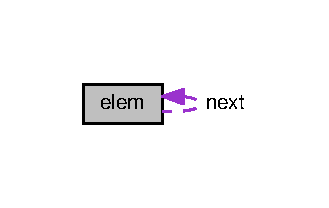
\includegraphics[width=158pt]{structelem__coll__graph}
\end{center}
\end{figure}
\subsection*{Attributi pubblici}
\begin{DoxyCompactItemize}
\item 
unsigned \hyperlink{structelem_aca409f3a7c1c9621b262a230c78ef37b}{col}
\item 
double \hyperlink{structelem_a52a0b099052bdf7611aa32acdb3f5449}{val}
\item 
struct \hyperlink{structelem}{elem} $\ast$ \hyperlink{structelem_ab9cf5c2e1c9a0ec2938275b90d39d5ca}{next}
\end{DoxyCompactItemize}


\subsection{Descrizione dettagliata}
Le matrici sparse di valori double sono rappresentate da un array di liste ciascuna delle quali rappresenta una riga. In ogni lista sono contenuti solo gli elementi non uguali a zero con il numero di colonna corrispondente.

Ad esempio la matrice

3.\+1 0 0 0 0 0 0 0 0 7.\+2 0 9.\+0

è rappresentata come

0 $\vert$ ------$>$(\mbox{[}0,3.\+1\mbox{]} , N\+U\+LL) 1 $\vert$ N\+U\+LL 2 $\vert$ ------$>$(\mbox{[}1,7.\+2\mbox{]} , --)--$>$( \mbox{[}3,9.\+0\mbox{]} ,N\+U\+LL)elemento della matrice sparsa 

\subsection{Documentazione dei membri dato}
\index{elem@{elem}!col@{col}}
\index{col@{col}!elem@{elem}}
\subsubsection[{\texorpdfstring{col}{col}}]{\setlength{\rightskip}{0pt plus 5cm}unsigned elem\+::col}\hypertarget{structelem_aca409f3a7c1c9621b262a230c78ef37b}{}\label{structelem_aca409f3a7c1c9621b262a230c78ef37b}
indice di colonna \index{elem@{elem}!next@{next}}
\index{next@{next}!elem@{elem}}
\subsubsection[{\texorpdfstring{next}{next}}]{\setlength{\rightskip}{0pt plus 5cm}struct {\bf elem}$\ast$ elem\+::next}\hypertarget{structelem_ab9cf5c2e1c9a0ec2938275b90d39d5ca}{}\label{structelem_ab9cf5c2e1c9a0ec2938275b90d39d5ca}
puntatore al prossimo elemento nella riga \index{elem@{elem}!val@{val}}
\index{val@{val}!elem@{elem}}
\subsubsection[{\texorpdfstring{val}{val}}]{\setlength{\rightskip}{0pt plus 5cm}double elem\+::val}\hypertarget{structelem_a52a0b099052bdf7611aa32acdb3f5449}{}\label{structelem_a52a0b099052bdf7611aa32acdb3f5449}
valore dell\textquotesingle{}elemento 

La documentazione per questa struct è stata generata a partire dal seguente file\+:\begin{DoxyCompactItemize}
\item 
\hyperlink{sparse_8h}{sparse.\+h}\end{DoxyCompactItemize}

\hypertarget{structsmatrix__t}{}\section{Riferimenti per la struct smatrix\+\_\+t}
\label{structsmatrix__t}\index{smatrix\+\_\+t@{smatrix\+\_\+t}}


{\ttfamily \#include $<$sparse.\+h$>$}



Diagramma di collaborazione per smatrix\+\_\+t\+:\nopagebreak
\begin{figure}[H]
\begin{center}
\leavevmode
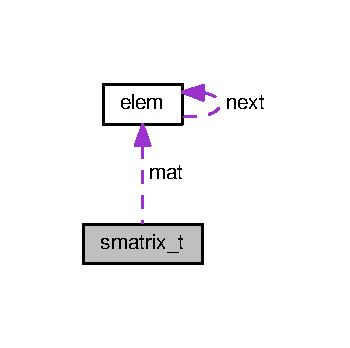
\includegraphics[width=168pt]{structsmatrix__t__coll__graph}
\end{center}
\end{figure}
\subsection*{Attributi pubblici}
\begin{DoxyCompactItemize}
\item 
\hyperlink{sparse_8h_a14aec81bdea9c2d34b666b7157117387}{elem\+\_\+t} $\ast$$\ast$ \hyperlink{structsmatrix__t_aa60ccb45be474ec81f6daab4fcdab2c4}{mat}
\item 
int \hyperlink{structsmatrix__t_ae0b8f31ddab7ed23ca14a46758291f37}{nrow}
\item 
int \hyperlink{structsmatrix__t_a7a7218430298fc18a42dfa43ecc41635}{ncol}
\end{DoxyCompactItemize}


\subsection{Descrizione dettagliata}
rappresentazione della matrice sparsa 

\subsection{Documentazione dei membri dato}
\index{smatrix\+\_\+t@{smatrix\+\_\+t}!mat@{mat}}
\index{mat@{mat}!smatrix\+\_\+t@{smatrix\+\_\+t}}
\subsubsection[{\texorpdfstring{mat}{mat}}]{\setlength{\rightskip}{0pt plus 5cm}{\bf elem\+\_\+t}$\ast$$\ast$ smatrix\+\_\+t\+::mat}\hypertarget{structsmatrix__t_aa60ccb45be474ec81f6daab4fcdab2c4}{}\label{structsmatrix__t_aa60ccb45be474ec81f6daab4fcdab2c4}
puntatore all\textquotesingle{}array delle righe \index{smatrix\+\_\+t@{smatrix\+\_\+t}!ncol@{ncol}}
\index{ncol@{ncol}!smatrix\+\_\+t@{smatrix\+\_\+t}}
\subsubsection[{\texorpdfstring{ncol}{ncol}}]{\setlength{\rightskip}{0pt plus 5cm}int smatrix\+\_\+t\+::ncol}\hypertarget{structsmatrix__t_a7a7218430298fc18a42dfa43ecc41635}{}\label{structsmatrix__t_a7a7218430298fc18a42dfa43ecc41635}
numero di colonne \index{smatrix\+\_\+t@{smatrix\+\_\+t}!nrow@{nrow}}
\index{nrow@{nrow}!smatrix\+\_\+t@{smatrix\+\_\+t}}
\subsubsection[{\texorpdfstring{nrow}{nrow}}]{\setlength{\rightskip}{0pt plus 5cm}int smatrix\+\_\+t\+::nrow}\hypertarget{structsmatrix__t_ae0b8f31ddab7ed23ca14a46758291f37}{}\label{structsmatrix__t_ae0b8f31ddab7ed23ca14a46758291f37}
numero di righe 

La documentazione per questa struct è stata generata a partire dal seguente file\+:\begin{DoxyCompactItemize}
\item 
\hyperlink{sparse_8h}{sparse.\+h}\end{DoxyCompactItemize}

%--- End generated contents ---

% Index
\backmatter
\newpage
\phantomsection
\clearemptydoublepage
\addcontentsline{toc}{chapter}{Indice}
\printindex

\end{document}
